\evenchapter{Généralisation cartographique et préparation des données}

\textit{Cette partie aborde le travail préparatoire d'environ cinq semaines.\footnote{Le déroulement du projet figure en annexe ??} La base de donnée topographique de la Polynésie Française comporte les couches produites pour l'échelle 1/5000 et doivent être généralisées pour s'adapter à des échelles plus petites allant jusqu'au 1/500 000.}




\section{Préparation des traitements}
\subsection{Inventaire des traitements et des outils à disposition}

Les deux logiciels utilisés pour le traitement des données, FME Workbench 2022.0 et ArcGIS Pro, présentent une gamme d'outils servant à la généralisation. Les opérations qui seront utilisées sont détaillées dans la figure XX. Les outils sont classés selon les types de généralisation en reprenant le vocabulaire de \cite{Mustiere2001} qui a proposé une classification de ces opérateurs.
Le travail a été majoritairement effectué avec ArcGIS PRO à l'aide de l'outil ModelBuilder. Des scripts sur FME ont aussi été utilisés notamment pour les courbes de niveau et la problématique que leur généralisation soit en accord avec les points côtés. 
L’utilisation du ModelBuilder permet de transmettre et modifier facilement le travail réalisé à la suite du stage. 

\subsection{Structuration des métadonnées}

Chacune des opérations de généralisation \footnote{Désignés comme un traitement dans ce rapport} prennent en amont des données de départ. Les métadonnées sont produites pour chaque traitements et explicitent les éléments suivants :
\begin{itemize}
\item Les données de départ 
\item La nature des traitements effectuées ( nom de l'algorithme employé, du logiciel utilisé ) avec leurs paramètres et l'objectif d'un tel traitement. Souvent, les paramètres des géotraitements sont adaptés à l'échelle ou à une étendue géographique bien précise ce qui est aussi mentionné.
\item les données d'arrivée généralisées
\item les limites du traitement ainsi des pistes d'améliorations suggérées
\end{itemize}

Les couches généralisées cumulent lorsque cela est possible, les objets adaptés aux différentes échelles. 
Une sélection peut se faire dans ce cas via la table attributaire et les champs ECHELLE\_MIN et ECHELLE\_MAX qui indiquent sur quel plage d'échelle chaque entités de la couche doit être utilisée.
La partie 2.2 présente ces traitements tandis que l'ensemble des métadonnées figure en annexe
 ?? avec le schéma de l'algorithme associé ( ModelBuilder d'ArcGIS ou modèle FME )



\section{Principaux traitements de généralisation}

\textit{Dans cette partie, les généralisations effectuées sont détaillées successivement et pour chaque type de couche. Des remarques concernant les choix de généralisation, leurs avantages et leurs limites figurent également. La quantité de travail est inégale entre les couches d'autant que comme on peut l'observer dans le tableau de l'annexe xx, certains couches d'entités souvent ponctuelles comportent un champ "importance" et ne nécessite pas de généralisation cartographique.}

\subsection{Les bâtiments}
\begin{center}
    \footnotesize
    \textbf{EDI\_BATI}
\end{center}
Puisqu'il s'agit de cartographier la Polynésie Française, le modèle doit s'adapter au mieux à la géographie des îles de la Polynésie. En effet, on observe souvent une concentration des bâtiments proches du littoral et à la fin des vallées. Il y a peu de maisons isolées (type fermes) au milieu de champs comme en métropole.

\begin{figure}[ht]
\centering
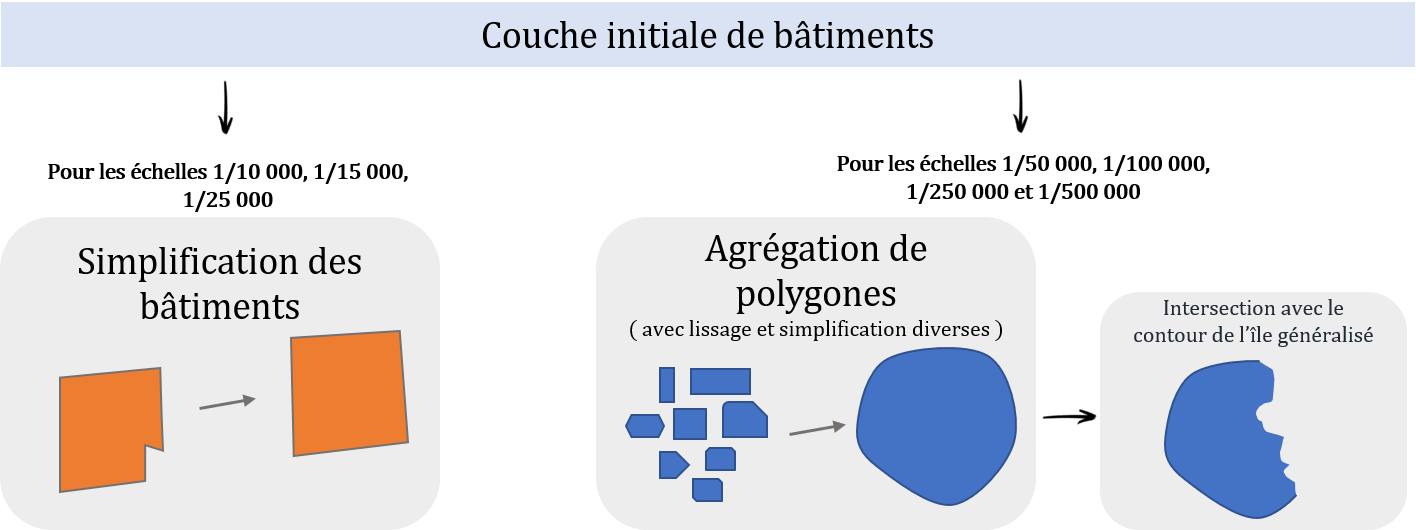
\includegraphics[width=\linewidth]{images/chap1/batiment_mb.png}
\caption{Explication schématique des traitements réalisés sur la couche EDI\_BATI}
\label{bati_mb}
\end{figure}

Les choix adoptés sont illustrés sur la figure \ref{bati_mb}. Le traitement \textbf{ Simplifier des bâtiments} est employé jusqu'à l'échelle 1/25000. C'est un traitement réalisé en dérivation ce qui signifie que le résultat pour chacune des échelles supérieures ou égales au 1/25 000 provient de la couche initiale calibrée pour le 1/5000. Il faut noter que l'outil \textit{"Simplifier les bâtiments"} d'ArcGIS propose d'éliminer les entités dont la superficie serait inférieure à une certaine valeur à définir. Cette option a été mise à profit pour supprimer les petits cabanons dans un premier temps puis les très petits bâtiments à des échelles inférieures. Sur la figure \ref{resultat_bati} (Carte A), on observe ces modifications de la géométrie ainsi que les suppressions de petits bâtiments. Tous les paramètres numériques des algorithmes font partie des métadonnées et se retrouvent dans l'annexe xx.

Pour les échelles inférieures ( du 1/500 000 au 1/50 000), la méthode est différente puisqu'elle s'appuie sur le traitement : \textbf{"Agréger les polygones"}. Il est non seulement possible de supprimer des entités trop petites mais aussi de gérer la taille des trous polygonaux. Comme l'illustre la figure  \ref{resultat_bati}, les trous polygonaux peuvent être pertinents au 1/50 000 (Carte B) mais le sont moins au 1/500 000 (Carte C).
dans cette gamme d'échelle, les traitements se font en série et par ordre d'échelle décroissante c'est à dire que la couche produite pour le 1/50 000 est à l'origine de celle produite pour le 1/100 000 et ainsi de suite. Pour assurer la cohérence de la cartographie et éviter que des agrégations de polygones ne viennent empiéter sur les lagons, un traitement supplémentaire ( cf model builder de l'annexe xx ) effectue l'intersection avec la la couche du contour de l'île adaptée. En effet, celle-ci étant aussi généralisée, l'intersection pour une échelle donnée se fait avec les entités adaptées à l'échelle.


\begin{figure}[ht]
\centering
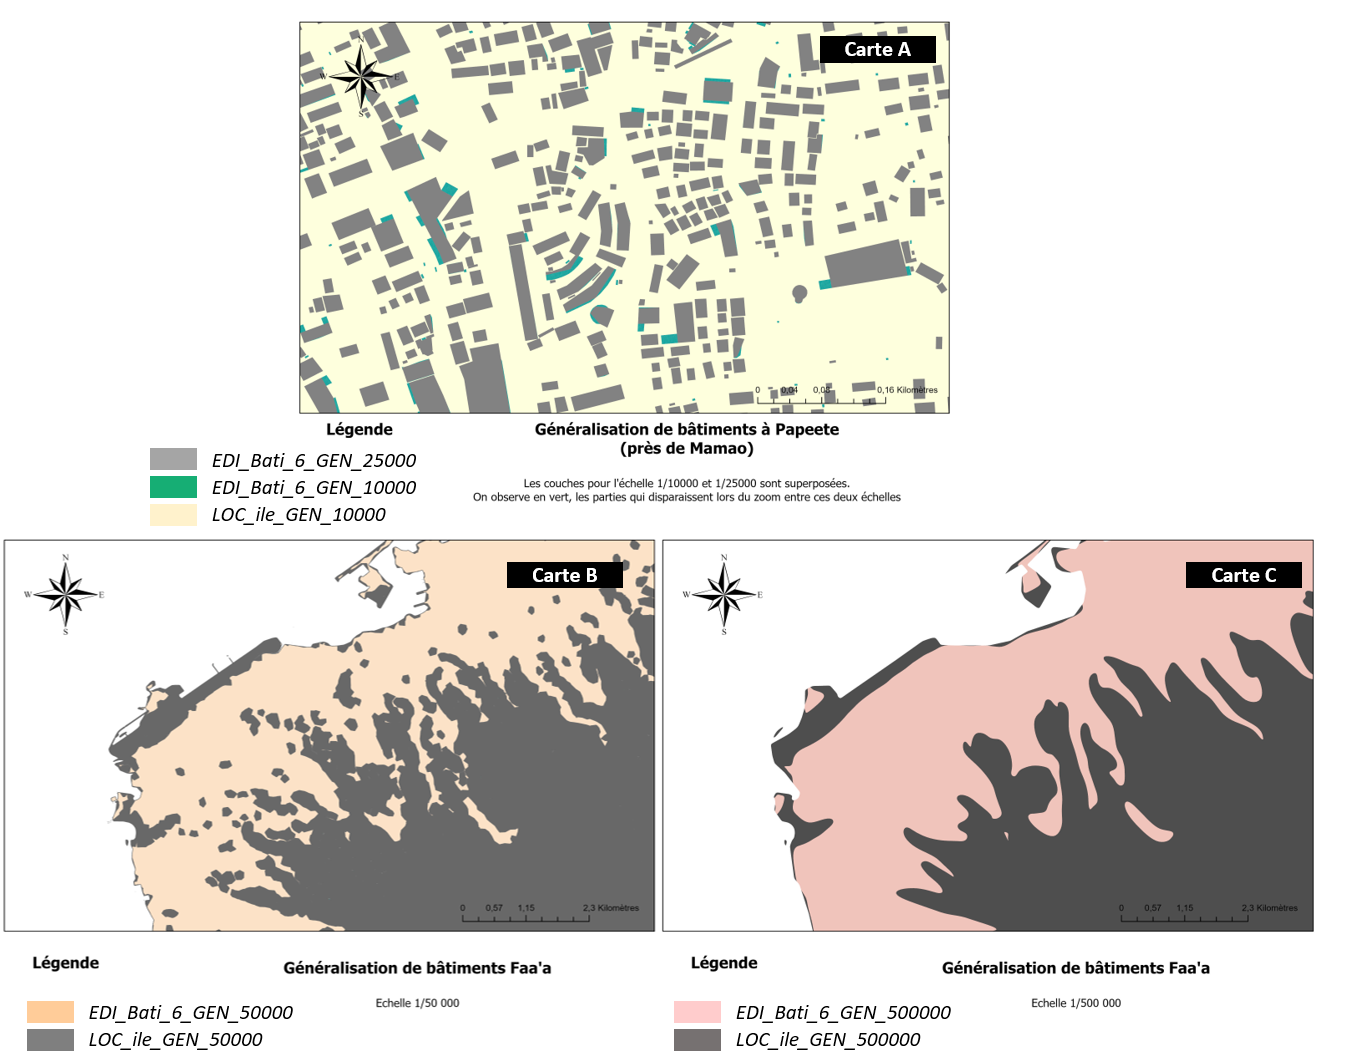
\includegraphics[width=\linewidth]{images/chap1/resultat_bati_bis.png}
\caption{Quelques résultats de généralisation sur la couche EDI\_BATI}
\label{resultat_bati}
\end{figure}

\begin{center}
    \textit{Quelles pistes d'amélioration ?}
\end{center}

Lors de la généralisation aux grandes échelles, il est parfois possible que des bâtiments se superposent. Les traitements sur ArcGIS permettent de signaler des conflits spatiaux avec un champ dédié. Cependant, le travail de gestion des conflits spatiaux n'a pas été fait car ces derniers étaient mineures. En effet les paramètres de simplification choisies restent relativement faibles et ne déforment pas suffisamment les bâtiments pour qu'un grand nombre d'entre eux se superposent. De plus, la suppression des petits cabanons évite de nombreux conflits spatiaux.

\subsection{Les constructions surfaciques}
\begin{center}
    \footnotesize
    \textbf{EDI\_CONSTRUCTION\_S}
\end{center}

Les constructions surfaciques sont généralisées de manière similaire à celle des bâtiments à la différence qu'elles ne sont jamais regroupées. Lorsque le point de généralisation qui correspond à l'échelle 1/25 000 est passé, alors la simplication de la géométrie est plus prononcée et le tri se fait de manière à ne garder que les entités d'intérêt. Tous les paramètres numériques utilisés figurent en annexe XX. On notera par exemple le choix d'une superficie minimale de 7000 m² pour l'échelle 1/50 000 de manière à ne conserver que les terrains de foot et autres constructions plus grandes tout en supprimant les terrains plus petits et plus nombreux qui ne serait pas lisibles sur la carte à cette échelle.

\textsc{Remarque :}
La présence des constructions surfaciques de grande ampleur peut se discuter à l'échelle 1/250 000. Il dépend notamment du support de la carte. S'il peut être pertinent de les placer sur une carte papier, leur présence se discute pour un support web multi-échelle. 

\subsection{Les limites administratives}

\begin{center}
    \footnotesize
    \textbf{LOC\_ile et LOC\_limite\_commune}
\end{center}

La couche LOC\_ile qui permet de connaître le contours des îles est composée d'entités surfaciques ( Une île représente un polygone ou un multi-polygone si elle est bordée de motus.)
La cellule topographie propose deux produits différents en ce qui concerne les communes.Le premier est une couche d'entités surfaciques correspondant aux communes tandis que le second est une couche d'entités linéaires faisant figurer les limites. Par ailleurs à Tahiti, le découpage administratif fait apparaître des regroupements de communes nommés "communes associées".\\

Les généralisations de ces deux couches, bien que leur géométrie soit différente, est similaire. Cela permet d'harmoniser les courbes de la carte. Pour ces deux couches, le traitement est le même pour toutes les échelles : il s'agit d'une simplication de ligne (ou polygone ) suivit d'un lissage. Les paramètres sélectionnés (voir annexe xx) sont choisis pour que le résultat soit approprié avec l'échelle.

En ce qui concerne les algorithmes, D-PK puis PAEK à décrire avec une figure

\subsection{Les lignes de relief}
\begin{center}
    \footnotesize
    \textbf{REL\_ligne\_relief}
\end{center}
L'annexe B décrit entre autres l'ensemble des catégories figurant dans la couche REL\_ligne\_relief. On observe de nombreux traits de reliefs. Certains sont à éliminer dès les premières échelles en dessous du 1/5000. C'est le cas notamment des éléments qui font partie de la catégorie \textit{Lignes caractéristiques}. 

En ce qui concerne les courbes de niveau, la mise en évidence des courbes maîtresses et l'équidistance de celles-ci ne change pas jusqu'au 1/ 25 000 où le besoin de précision est extrêmement important. Il est à noter comme précisé dans la partie 2.1.2, que la carte au 1/25 000 est une carte topographique dont l'utilité comme c'est le cas en métropole peut être celle de la randonnée et de l'exploration. En effet, l'échelle est trop importante pour être utilisée pour le cadastre mais permet de couvrir avec précision une zone suffisamment grande pour visualiser quelques randonnées dans leur intégralité.

La généralisation pour les échelles plus petites nécessite des algorithmes complexes dans la mesure où les points côtés ne doivent pas être faussées et les lignes ne doivent pas s'intersecter. L'utilisation d'algorithmes de simplification de lignes comme ceux de Wang-Muller ou de Douglas-Peucker ne font pas l'affaire. La technique consiste à utiliser le généralisateur de Sherbend disponible sur le logiciel FME. 

Comme on peut le retrouver dans la documentation FME ainsi que dans les exemples \cite{sherbend}, le généralisateur de Sherbend ( SherbendGeneralizer) prend en entrée des lignes et des points et généralise avec un algorithme complexe et chronophage qui s'appuie sur celui de Douglas-Peucker de manière à ce que la généralisation ne change pas la position des points par rapport aux lignes ce qui s'avère intéressant pour maintenir la justesse de la carte.Les problèmes d'intersection de lignes sont aussi gérés par cet algorithme. Son utilisation à l'aide d'un script FME semble donc adpatée pour la généralisation des courbes de niveau au 1/50000\footnote{Aux échelles inférieures, les courbes de niveau n'ont pas été placées. Ce choix est inspiré de celui fait par l'IGN lors de la réalisation de la carte de TAHITI en 1988. Ce choix est discutable car le produit Plan IGN consultable sur le géoportail fait figurer des courbes de niveau. Par ailleurs, les courbes de niveau, qui permettent de mieux se répérer peuvent être un élément intéressant pour un portail web et d'une carte multi-échelle. La carte de l'IGN de 1988 compense cette absence de courbes de niveau par un relief très prononcé. (voir annexe \ref{sherbend})}.

\begin{figure}[ht]
\centering
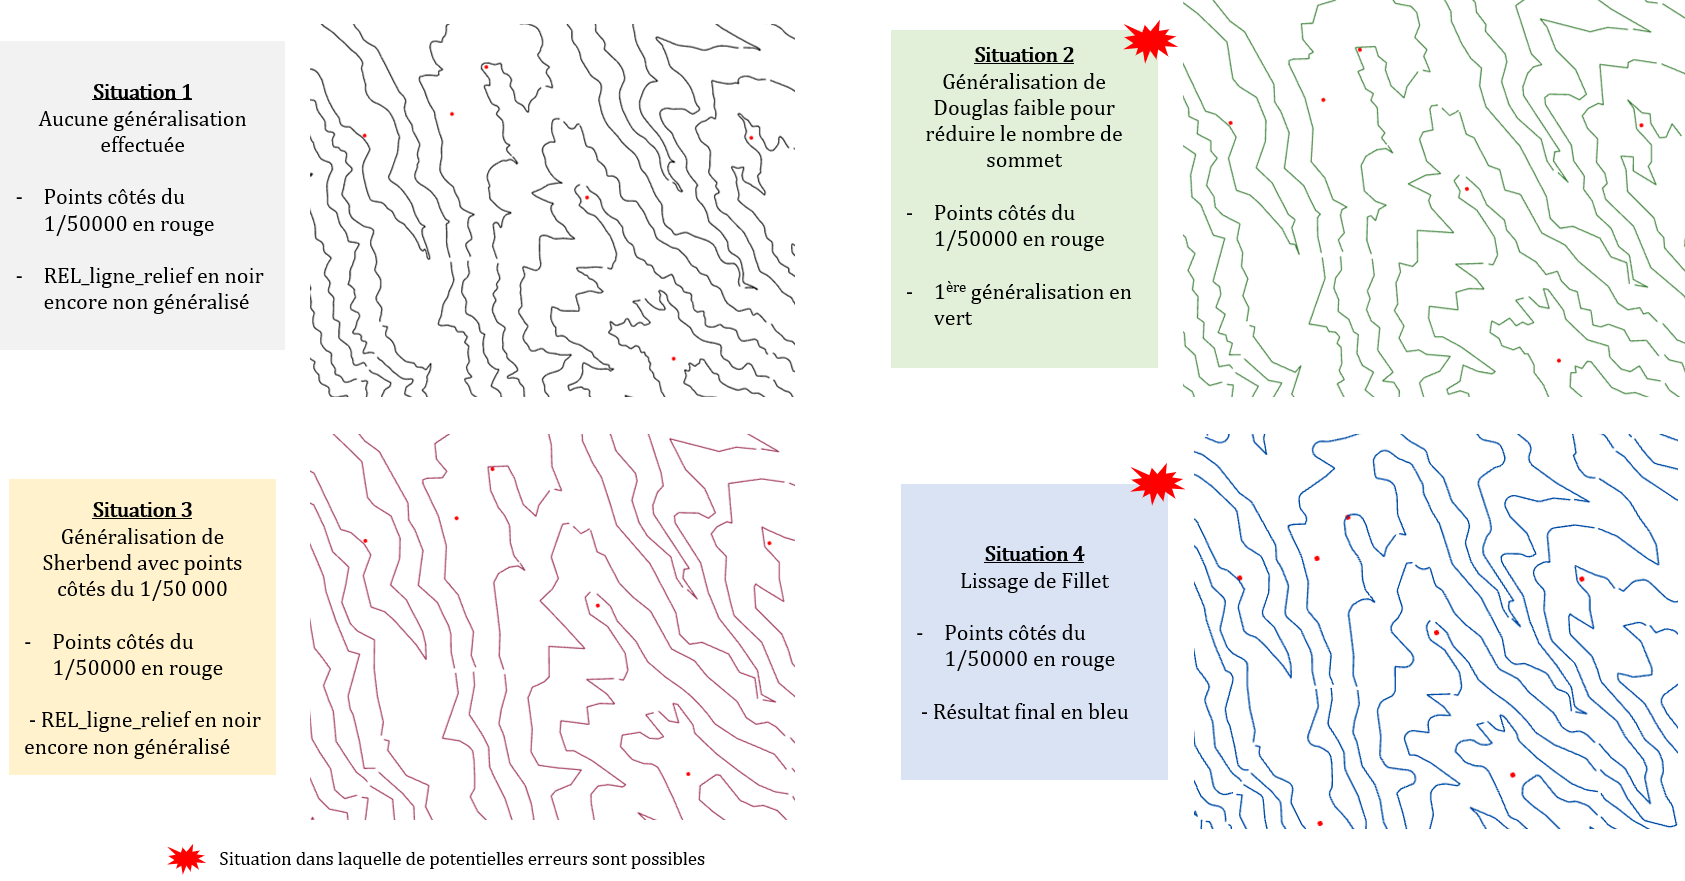
\includegraphics[width=\linewidth]{images/chap1/sherbend.png}
\caption{Quelques résultats de généralisation sur la couche EDI\_BATI}
\label{situation_sherbend}
\end{figure}
La figure \ref{situation_sherbend} décrit les étapes du processus de généralisation. Cette solution n'est pas optimale et de potentielles erreurs sont possibles et seront décrites dans ce rapport
Les données de départ sont les courbes de niveau non généralisée avec les points côtés  du 1/50000, c'est à dire ceux qui seront affichés sur la carte avec les courbes de niveau généralisées.
Un traitement préalable de sélection attributaire permet de ne garder que les courbes de niveau dites maîtresses (équidistantes de 100 m). Voici le descriptif des traitements ( illustrés par la figure \ref{situation_sherbend})
\begin{itemize}
\item Le premier traitement du script FME est une généralisation assez fine avec l'algorithme de Douglas-Peuker.  Ce traitement s'avère nécessaire pour permettre d'appliquer par la suite le traitement \textit{"SherbendGeneralizer"}. S'il n'est pas effectué , les temps de calculs seront beaucoup trop longs et cela d'autant plus si la généralisation ne s'applique sur toutes les courbes de niveau et non pas seulement comme c'est le cas ici sur les courbes maîtresses. Cependant, travailler sur des plus petites zones permet d'éviter cette étape. Il faut aussi noter que la généralisation est à priori assez fine et bien qu'il soit possible de fausser certains points avec cette étape, le risque reste faible avec les paramètres choisis ( paramètres détaillés dans l'annexe xx). A l'issu de ce traitement, le résultat est illustré par la Situation 2 de la figure \ref{situation_sherbend}
\item Le deuxième traitement est la généralisation de Sherbend à proprement parlé. Elle est paramétrée de manière à éviter les écueils qui peuvent survenir dans le cas d'une généralisation classique ( intersections de lignes et incohérence des courbes de niveau avec les points côtés). La simplification de ligne doit amener à la suppression des détails qui surchargeraient la carte au 1/50 000. A l'issu de ce traitement, le résultat est illustré par la Situation 2 de la figure \ref{situation_sherbend}
\item Enfin, le lissage est une dimension absente de l'algorithme précédent. Or l'absence de lissage est problématique pour le rendu cartographique. Cependant, comme c'était le cas dans l'étape 1, retoucher à la la géométrie des courbes de niveau signifie commettre potentiellement des erreurs sur les points côtés et sur la géométrie. Ainsi, pour limiter les potentielles erreurs, c'est un lissage de Fillet qui est choisi. Le principe de cet algorithme est d'arrondir les points anguleux d'une ligne avec comme paramètre un rayon (fixé à 0, la géométrie de la ligne est inchangée). Toute la problématique est donc de pouvoir produire un résultat suffisamment lissé sans générer d'erreurs. Enfin, la généralisation se tremine par la création d'un champ nommé \textit{"Classe\_1\_2" }qui établit une nouvelle classification des courbes obtenues. En effet, ces courbes, équidistantes de 100m, sont des courbes maitresse dans le classement initial. Un  nouveau classement établit des courbes maitresse tous les 500m.\\
\end{itemize}
\textsc{Remarques et pistes d'amélioration :}\\
Il est possible de ne pas commettre la première erreur en amont du généralisateur de Sherbend par un découpage plus détaillé des courbes de niveaux notamment sur Tahiti où leur nombre est important.

Pour ce qui est du lissage final (étape qui semble incontournable pour la lisibilité de la carte), il faudrait pouvoir mettre en place un système de contrôle de la géométrie et de la position des points côtés en fin d'algorithme de manière à prévenir des potentielles erreurs mais cette dimension n'a pas été abordée au cours de ce stage.



\subsection{Les tronçons hydrologiques et les surfaces d'eau}

La généralisation des cours d'eau est une étape délicate dans le processus de cartographie. En effet, à de petites échelles, une modification de la géométrie peut entraîner des conflits avec les autres couches, notamment les bâtiments. On ne saurait tolérer des inexactitudes géométriques allant jusqu'à la superposition de ces deux couches.Par ailleurs, une autre problématique correspond à la cohérence des surfaces d'eau avec les tronçons hydrologiques. Ainsi, les cartes réalisées au cours de ce projet font figurer des échelles 1/25 000 aux échelles 1/5000, la couche la plus détaillée de tronçons hydrographiques ainsi que la couche la plus détaillée de surface d'eau. La généralisation à effectuer entre ces échelles est simplement une sélection dans la table attributaire visant à éliminer certaines rigoles ou caniveaux trop insignifiant pour des échelles comme le 1/25 000. \footnote{Concernant ces couches, le travail de généralisation a donc été mineur jusqu'au 1/ 25 000. Jusqu'à cette échelle, la précision importante n'empêche pas la production d'une carte lisible, adaptée et cohérente. On notera  tout de même le cas de Raiatea (Île sous le Vent) où le nombre de tronçons hydrologiques répertoriés dans la base est très élevé ce qui surcharge énormément la carte au 1/25 000 alors que ça n'est pourtant pas le cas sur Tahiti}


\begin{center}
Comment généraliser ces deux couches à des échelles inférieures ?
\end{center}

\begin{center}
    \footnotesize
    \textbf{HYD\_troncon\_eau\_L}
\end{center}
Un possibilité pourrait être de considéré à partir du 1/50 000 uniquement les cours d'eau catégorisés pour cette échelle. Cependant, aucun champ de la base de donnée ne classe les cours d'eau. Une tentative a été faite en ne sélectionnant que les cours d'eau nommé car ces derniers sont jugés suffisamment important. Cependant cette méthode ne fonctionne pas car la base de donnée présente de nombreuses portions de cours d'eau non nommé. C'est donc une tout autre méthode qui doit être envisagée. Il s'agit d'une solution amenée à être provisoire en cas de restructuration future de la BDD.

Pour les petites échelles, les tracés hydrographiques se font à partir d'un MNT sur lequel des traitements hydrologiques ont été réalisés. Les documents de l'annexe xx détaillent ces traitements et les quantifient. Le principe est l'enchaînement de traitements sur le MNT raster pour en extraire les pixels correspondant à des rivières et les convertir en une couche vecteur. Une jointure spatiale en fin d'algorithme permet d'ajouter la toponymie des rivières. On notera que cette méthode peut être considérée comme provisoire si la base de donnée vient à être modifiée.

\begin{figure}[ht]
\centering
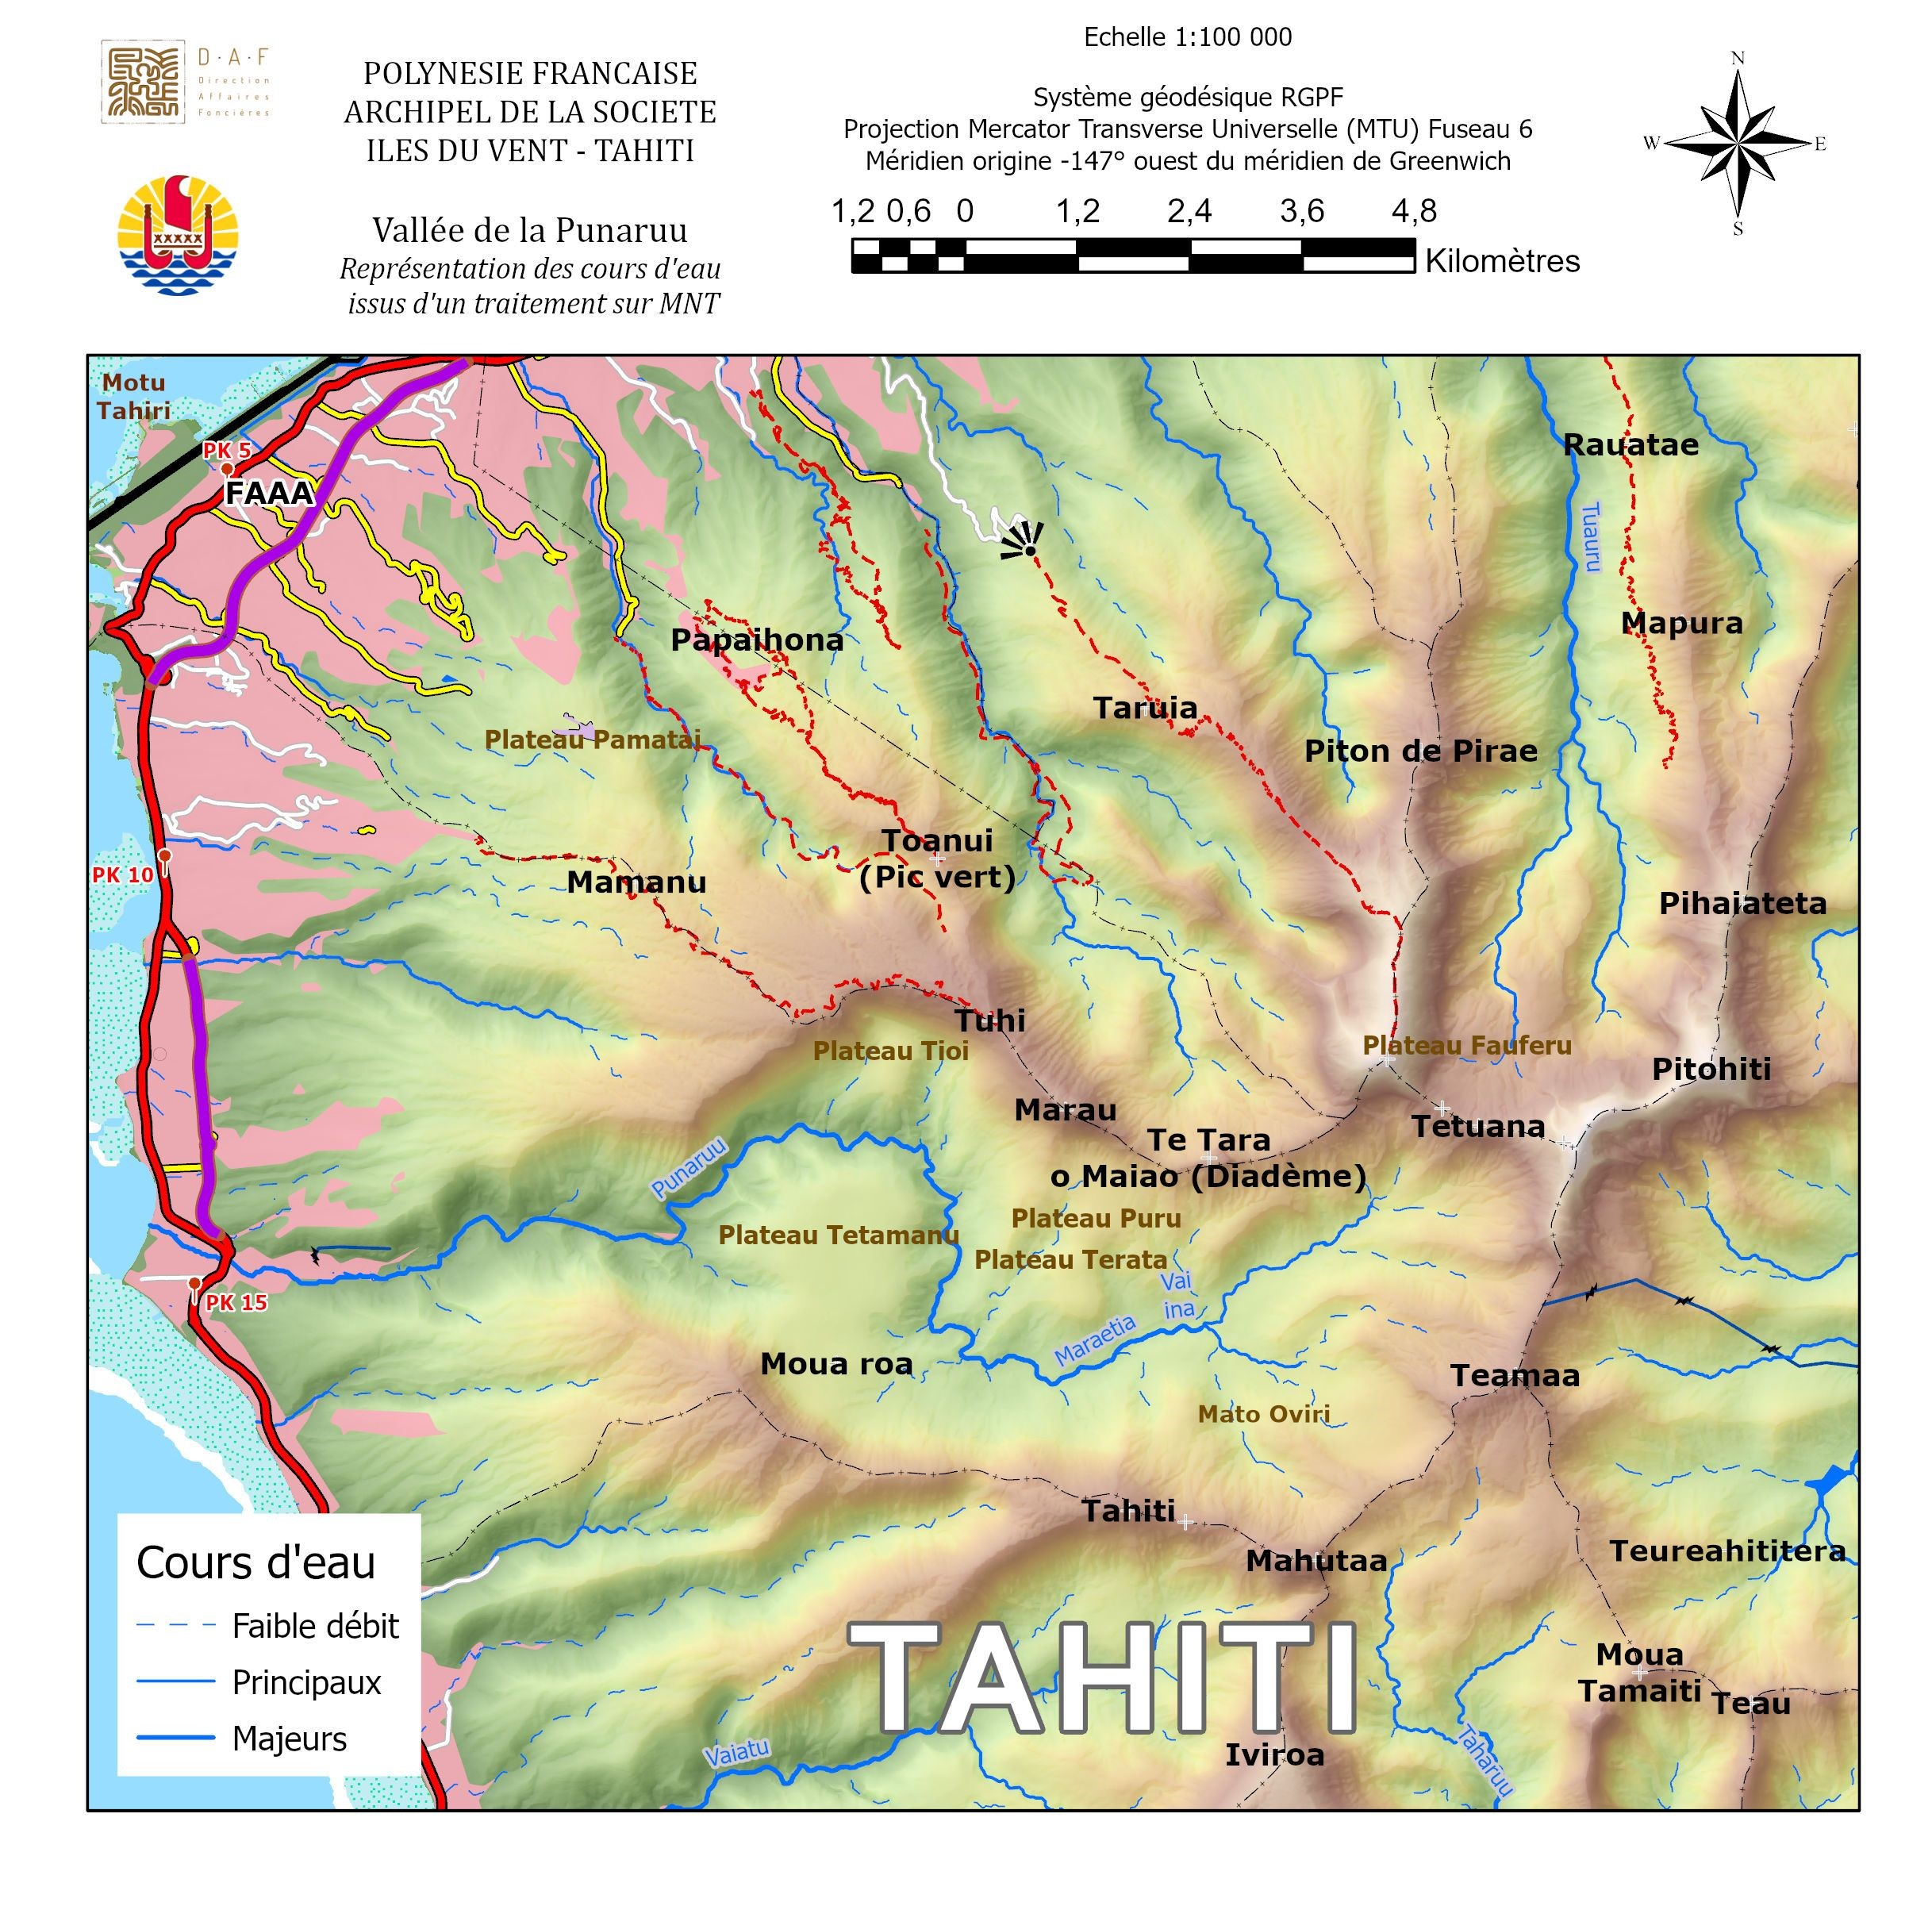
\includegraphics[scale=0.7]{images/chap1/carte_eau.jpg}
\caption{Représentation des cours d'eau issus du traitement sur MNT}
\label{carte_eau}
\end{figure}
 

\begin{center}
    \footnotesize
    \textbf{HYD\_surface\_eau\_S}
\end{center}
Ce traitement complémentaire de simplification des polygones hydrologiques se base sur des simplifications de polygones ( avec élimination des entités de surface trop faible). Le modèle de ce traitement ainsi que les paramètres sont présents dans l'annexe xx

\section{Remarques et traitements secondaires}
\subsection{La voirie et sa catégorisation}
\begin{center}
    \footnotesize
    \textbf{VOI\_troncon\_route\_L, VOI\_limite\_route\_L et VOI\_mobilier\_route\_P }
\end{center}
La généralisation réalisée pour les couches qui concernent la voirie correspondant davantage à une restructuration du champ \textit{"classement" }pour avoir un nombre de catégories adapté à l'échelle. Parmi les opérations effectuées, on compte des suppressions d'entités, des groupements ainsi que des créations de champs. Ce travail est indissociable de la symbologie choisie qui fait l'objet de la partie suivante. Le travail s'est essentiellement porté sur la couche \textit{"VOI\_troncon\_route\_L"}. La couche \textit{"VOI\_limite\_route\_L"} devient quand à elle inutilisable pour des échelles trop petites tandis que la couche \textit{"VOI\_mobilier\_route\_P"} n'est utilisée que pour l'affichage des bornes. kilométriques\footnote{Il s'agit simplement d'une sélection attributaire étendue à une sélection sur le kilométrage de la borne (sélection tous les kilomètres ou tous les cinq kilomètres)}

{\color{magenta}PARTIELLEMENT REDIGE Le schéma XX ici ou en annexe en fonction de la place présente les catégories retenues à travers les différentes échelles.} On notera les difficultés pour mettre en évidence la route traversière de Tahiti. Une des propositions envisagées serait de créer dans la base de donnée un champ spécial pour les routes traversières présentes sur de nombreuses îles hautes en Polynésie.


\subsection{Remarques sur les couches ponctuelles}

Les couches d'entités ponctuelles nécessitent souvent une généralisation par sélection attributaire selon un champ \textit{"importance"} dédié. Les couches ponctuelles brièvement évoquées précédemment sont les couches de points côtés et de mobilier de route. Une couche ponctuelle qui a fait l'objet d'un travail de réflexion important est la couche \textbf{HYD\_point\_eau\_P}. On y retrouve notamment les sources, fontaines et cascades et la base de donnée ne fait pas encore figurer de champ permettant la généralisation. Différentes possibilités ont été envisagées pour généraliser la couche :
\begin{itemize}
\item Un traitement d'agrégation regroupant par exemple les cascades proches selon le centroïde. Cependant ce traitement entraîne des inexactitudes géométriques\footnote{qui peuvent néanmoins être tolérées}, mais aussi un problème dans la symbologie : faut-il mettre un symbole proportionnel au nombre de cascades regroupées ? comment négliger les cascades insignifiantes ?
\item La création d'un champ hauteur pour chacune des cascades répertoriées. La généralisation consisterait alors à trier en ne gardant que les plus grandes cascades lors du changement d'échelle. Cependant, une cascade n'est pas forcément signifiante uniquement par sa taille. Elle peut l'être aussi par son débit (souvent variable) ou sa position géographique. Toutes ces informations qui contribueraient à la construction d'une base de données extrêmement précises sont difficilement **renseignables** sur le nombre très conséquent de cascades que comporte la Polynésie.
\item la création d'un champ importance propre à chaque entité. Cette  solution semble la meilleur bien que contrairement à la précédente, elle n'apporte pas de précisions supplémentaires sur la donnée. Il s'agit cependant d'un vaste travail nécessitant potentiellement l'appel à des sociétés extérieures.\\
\end{itemize}

\textsc{Remarques diverses:}
\begin{itemize}
\item Les couches de Toponymes et de PAI sont des couches ponctuelles déjà généralisées. Elles servent pour l'étiquetage qui sera évoqué dans la partie suivante.
\item Certaines couchent ne sont pas généralisés (absence de modifications géométriques et de restructuration des champs pour la symbologie), soit parce qu'elles ne sont pas utilisées dans la cartographie (voir tableau de l'annexe xx) . Une des problématique non résolue de ce travail est la généralisation des couches d'occupation du sol notamment en zone urbaine. Pour rendre la carte lisible, les simplifications effectuées seront détaillées dans le chapitre suivant. 
\end{itemize}





